As a part of the course Experts in Team (EiT) at NTNU, five students were put in a group to collaborate on a project. This team (us) was a part of the virtual reality village of EiT, and came up with the following problem statement:

\setlength{\parskip}{-0.15in}
\begin{center}
	\em How can you make an affordable and usable prototype\\
	for head tracking to be used for virtual reality?
\end{center}

We solved this problem by first doing a preliminary study followed by design and implementation of the solution. In the preliminary study, several technical and theoretical subjects were investigated. The mathematics behind estimation of object position from pictures were elaborated. We looked at the available technology for connecting a high definition camera to a PC and reading the images from it. We studied the properties of infrared light. We looked at and tested the Nintendo Wii and its Wiimotes. Lastly, potential areas of use for a solution was described.

\setlength{\parskip}{0.1in}

Then, a specification of the requirements was carefully crafted. The specification was the basis for the design of the solution. This design specifies how the components of the system is constructed and how they are connected. The components of the system make up a pipeline:

\begin{figure}[h]
\centering
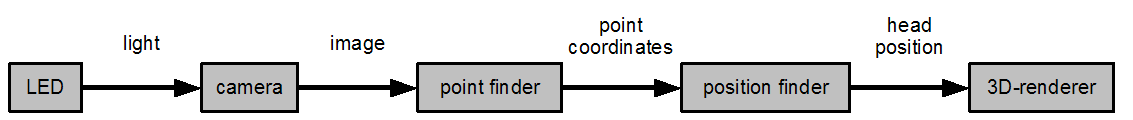
\includegraphics[width=\textwidth]{graphics/main_design_english.png}
\end{figure}

The LED-component is a set of infrared LEDs that are attached to the user's head. These transmit light that is captured by a high definition camera. The image from this camera is read by our point finder software that attempts to locate the coordinates of the bright dots in the image where the LEDs are. These coordinates are transferred to the position finder software which uses them to estimate the position of the user's head. This head position is then used by the 3D-renderer software to display a 3D-scene on a screen where the viewpoint is mapped to the head position.

The implementation was done by acquiring a Panasonic high definition digital camera and connecting this to a PC with an HDMI-card. In addition, a headset with infrared LEDs was constructed. For the software part, the point finder, posistion finder and 3D-renderer was written in Java with bindings to native machine code for the 3D-rendering part.

We ended up with an adaptive solution. In addition to using the high definition camera connected to a PC by HDMI, one can use a Nintendo Wiimote by wireless Bluetooth network. Even {\em two} Wiimotes can be used for improved tracking. The system follows the requirements and design specifications. It provides virtual reality by tracking the position of the user's head and displaying a 3D-scene on a screen in front of the user. The viewpoint in this scene is moved to match the position of the head. This creates the sensation of looking into a real room through the sceen.

As for weaknesses of the system, we mention that the high definition camera turned out to show a latency of about half a second before its images being available to read. In short, the camera is not meant for real time video capture. Further, the LED-headset we constructed is flawed when it comes to handling rotation of the head and battery life time.

When it comes to strengths, we would like to point out that the high definition of the camera makes it possible to detect movement even far away from the camera. The possibility of using two Wiimotes for tracking gives the advantage of only one light being needed on the head on the user, which makes the tracking rotation invariant. The solution is adaptive, portable and reusable. It is adaptive because of its many configuration options. It is portable because of being written in the system indepented language Java. And it is reusable because of being split into components with low coupling between themselves.

The hardware cost of the solution is below 10 000 NOK. It is easy to set up and use and provides a strong sensation of reality. Thus, we conclude that it is possible to create such an affordable and usable system for head tracking as in the problem statement.